\chapter{粒子、波與解析度所需的能量}

\section{粒子還是場？}

粒子物理學研究什麼？粒子---但這個答案立刻引出一個古老的問題：自然界是離散的嗎？這裡的「離散」是指物質由彼此分開、不可再分的單位構成，和「圓滑得體」毫無關係。希臘詞\emph{atom}的意思是「不可分割」，儘管如今稱為原子的物體可以再分。目前，\emph{粒子}將泛指離散的單位。

與此相對的是連續體的圖像。物質不再是彼此分離的部分所構成的集合，而是連續地散布在空間中。描述這種圖像，自然要用場的語言。場是位置的函數：物質的密度是一種場，電場和磁場也是場。後兩者決定帶電粒子的運動方式，但在經典觀點中，場本身被視為連續分布於空間。

不宜過度拘泥於這些觀念在歷史上的先後次序。這樣排列有助於呈現論證的邏輯，卻不代表它是可靠的年代順序。粒子的語彙包括原子、分子、碰撞和局域物體；連續體的語彙則包括場和連續變化的性質。哪一種圖像才正確？量子力學使兩者都不可能完全正確，但也使兩者都不可能全然錯誤。

這裡的討論會盡量自成一體，不過後續論證仍會用到量子力學、經典力學、狹義相對論和電磁學。眼前的問題比較簡單：最初是什麼使人們相信物質確實是離散的？

\section{物質離散性的化學證據}

至少在這套邏輯論述中，最初有力的證據來自化學，而非物理學。這種區分其實是人為的：化學在很大程度上就是原子與分子的物理學。道耳頓比較不同物質中相同數目的分子之質量。要確認樣本所含分子數相同，本身就是一大難題。此處會提到阿伏伽德羅；一莫耳所含的分子數就是阿伏伽德羅常數。若只是比較分子數相同的樣本，並不需要知道這個數的實際值。

引人注目的規律是：各物質的莫耳質量約為氫的莫耳質量的整數倍。這些倍數通常不是\(3/2\)、\(\pi\)或任意實數，而是接近整數的數。舉例來說，碳-12的質量約相當於十二個以氫為基準的質量單位。這強烈暗示物質是由質量幾乎相同的基本單位反覆組成。

現代的解釋消除了這個謎團。普通原子由質子、中子和電子構成。電子質量只有質子或中子的大約兩千分之一，因此對原子質量的貢獻很小。質子和中子幾乎承載了全部質量，而兩者的質量差遠小於百分之一。普通氫的原子核只有一個質子，因此原子或分子的質量約為氫尺度核質量的整數倍。這只是近似說法：質子和中子的質量並不完全相同，電子也有少量貢獻。儘管如此，這種近似整數的規律仍揭示了物質由離散成分構成。

後來，人們理解到分子是由原子組合而成。十九世紀的化學家辨認出約一百種原子，並將它們歸類為元素；若按基本的計數方式，約有九十二種元素天然存在，若再區分同位素，種類還會更多。週期表並不是按樸素的想法，簡單地重複相同大小的區塊，但它將這些不同物種整理了起來。在當時，各種元素本身看起來就是基本構成單位。愛因斯坦1905年的研究提供了定量方法，使物質的分子理論得到更有力的確立；不過，在此之前，化學證據已使原子圖像相當令人信服。

十九世紀末，這個看似終點的圖像不再成立。電子被發現，放射性也揭示了「元素就是基本單位」的圖像無法解釋的現象。放射性在微觀尺度上，已包含許多後來成為核物理與粒子物理核心的問題。

\section{放射性與分離的束流}

確切的歸屬和年代順序並不明確。一般會暫且將這項觀察歸於貝克勒爾：放射性物質恰好放在照相底片附近，並使底片受到影響，彷彿有不可見的輻射照射它。與其只把底片曝光視為受損，不如追問究竟是什麼到達了底片。瑪麗·居里後來的許多研究也屬於這段歷史，但若要理解實驗的邏輯，無須精確劃分早期各項發現的歸屬。

把材料放在厚實鉛塊的深處，並留出一條通往照相底片的窄通道。鉛的密度高，適合用來遮蔽輻射；通道則會準直逸出的輻射。底片上出現的不是一片模糊曝光，而是一個局部斑點，顯示輻射形成了有方向的束流。就這套論述的邏輯而言，這是第一束粒子束，雖然此時還不知道束流的本質。

接著讓準直後的輻射通過一個與軌跡平面垂直的磁場。曝光分成三支：一支不偏轉，繼續直行；另兩支向相反方向彎曲，而且偏轉量不同。電荷符號反轉時，磁力方向也會反轉，因此向相反方向彎曲的兩支表現出相反的電荷；直行的一支則表現為中性輻射。\footnote{此示意圖重現了講課影片中00:14:34至00:19:31之間畫出的圖。}

\begin{figure}[h]
\centering
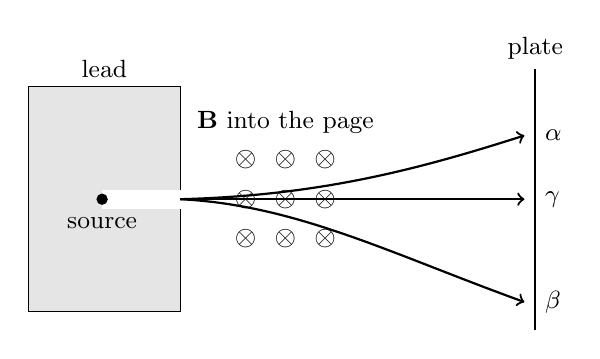
\begin{tikzpicture}[scale=0.92]
\draw[fill=gray!20] (0,-1.55) rectangle (2.1,1.55);
\draw[fill=white,draw=none] (1.02,-0.13) rectangle (2.12,0.13);
\draw[fill=black] (1.02,0) circle (0.07);
\node[below] at (1.02,-0.12) {\small source};
\node[above] at (1.05,1.55) {\small lead};
\foreach \x in {3.0,3.55,4.1}
  \foreach \y in {-0.55,0,0.55}
    \node at (\x,\y) {\(\otimes\)};
\node[above] at (3.55,0.78) {\small \(\mathbf B\) into the page};
\draw[thick] (7,-1.8) -- (7,1.8);
\node[above] at (7,1.8) {\small plate};
\draw[thick,->] (2.1,0) -- (6.85,0);
\draw[thick,->] (2.1,0) .. controls (4.0,0.05) and (5.35,0.40) .. (6.85,0.88);
\draw[thick,->] (2.1,0) .. controls (3.7,-0.08) and (5.0,-0.75) .. (6.85,-1.42);
\node[right] at (7,0.88) {\small \(\alpha\)};
\node[right] at (7,0) {\small \(\gamma\)};
\node[right] at (7,-1.42) {\small \(\beta\)};
\end{tikzpicture}
\caption{橫向磁場中的準直放射性束流。中性成分不偏轉；帶相反電荷的成分則向相反方向彎曲，且偏轉量不同。}
\end{figure}

這三種成分分別稱為阿爾法、貝塔和伽馬。用現代術語來說，
\begin{equation}
\begin{aligned}
\beta\text{-radiation} &= \text{electrons},\\
\alpha\text{-radiation} &= \text{helium nuclei},\\
\gamma\text{-radiation} &= \text{photons}.
\end{aligned}
\end{equation}
阿爾法粒子含有兩個質子和兩個中子，因此質量數為四。在道耳頓近似的整數序列中，氦因此會排在第四位：相當於四個氫尺度的核質量單位。貝塔射線是帶負電的電子，人們早已從陰極射線實驗中認識電子。伽馬射線不帶電。

若放射源足夠稀薄，且探測器能分辨個別的到達事件，看似連續的曝光就會呈現為一連串分開的事件：閃一下、再閃一下、又閃一下。貝塔、阿爾法和伽馬輻射也都可以如此觀測。蓋革計數器能呈現這種情形，至於最早的裝置是否確實在這種條件下操作，則是另一回事。每種成分都是以離散的束包抵達。伽馬射線仍是個謎：它是中性的，卻一次只探測到一個事件。伽馬輻射是能量極高的光，而普朗克、尤其是愛因斯坦，將光與量子聯繫起來。不過，在面對這個結論之前，必須先認真看待光具有波動性的經典證據。

\section{光的經典波動性}

在經典物理中，光是連續性的典型例子。它由電場和磁場構成，並以連續波的形式傳播。牛頓曾支持微粒說，但波動實驗使波動說取而代之。電荷振盪會產生電磁輻射。宏觀天線可以發射無線電波、微波、紅外線、可見光或紫外線；原子內部運動的電荷也相當於一支天線。所發出的輻射可以使照相底片曝光。

單狹縫提供了波動行為的初步線索。如果光是子彈流，穿過小孔後應會形成邊緣清晰、準直的光點。然而，實際照明會擴散成一片模糊區域。不過，光的擴散本身還不足以定論，因為也可以設想粒子受到孔徑邊緣的力而偏轉。

雙狹縫提供了更明確的檢驗。兩束彼此獨立的粒子流會形成兩片重疊的散布區域，重疊處或許最亮。波的表現則不同：一個狹縫傳來的波峰可以遇上另一個狹縫傳來的波峰，彼此增強；波峰也可以遇上波谷，彼此抵消。因此，螢幕上會出現明暗相間的條紋，其中甚至有些暗處，若只有任一狹縫開啟，本來都會被照亮。\footnote{此示意圖重現了講課影片中00:25:00至00:29:49之間畫出的孔徑與干涉圖。}

\begin{figure}[h]
\centering
\resizebox{\linewidth}{!}{%
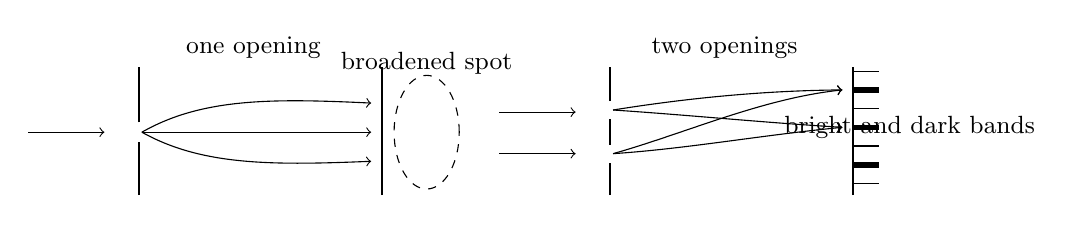
\begin{tikzpicture}[scale=0.88]
\begin{scope}
\draw[->] (-0.3,1.06) -- (0.8,1.06);
\draw[thick] (1.3,0.15) -- (1.3,0.92);
\draw[thick] (1.3,1.20) -- (1.3,2.0);
\draw[thick] (4.8,0.15) -- (4.8,2.0);
\draw[->] (1.34,1.06) .. controls (2.2,1.55) and (3.2,1.55) .. (4.65,1.48);
\draw[->] (1.34,1.06) -- (4.65,1.06);
\draw[->] (1.34,1.06) .. controls (2.2,0.58) and (3.2,0.58) .. (4.65,0.64);
\draw[dashed] (5.45,1.06) ellipse (0.47 and 0.82);
\node at (2.95,2.28) {\small one opening};
\node at (5.45,2.05) {\small broadened spot};
\end{scope}
\begin{scope}[xshift=6.8cm]
\draw[->] (-0.3,1.35) -- (0.8,1.35);
\draw[->] (-0.3,0.75) -- (0.8,0.75);
\draw[thick] (1.3,0.15) -- (1.3,0.62);
\draw[thick] (1.3,0.88) -- (1.3,1.25);
\draw[thick] (1.3,1.51) -- (1.3,2.0);
\draw[thick] (4.8,0.15) -- (4.8,2.0);
\draw[thin] (4.8,0.32) -- (5.18,0.32);
\draw[line width=2pt] (4.8,0.59) -- (5.18,0.59);
\draw[thin] (4.8,0.86) -- (5.18,0.86);
\draw[line width=2pt] (4.8,1.13) -- (5.18,1.13);
\draw[thin] (4.8,1.40) -- (5.18,1.40);
\draw[line width=2pt] (4.8,1.67) -- (5.18,1.67);
\draw[thin] (4.8,1.94) -- (5.18,1.94);
\draw[->] (1.34,0.75) .. controls (2.4,0.82) and (3.5,1.02) .. (4.65,1.13);
\draw[->] (1.34,1.38) .. controls (2.4,1.31) and (3.5,1.20) .. (4.65,1.13);
\draw[->] (1.34,0.75) .. controls (2.4,1.05) and (3.5,1.55) .. (4.65,1.67);
\draw[->] (1.34,1.38) .. controls (2.4,1.55) and (3.5,1.66) .. (4.65,1.67);
\node at (2.95,2.28) {\small two openings};
\node at (5.62,1.13) {\small bright and dark bands};
\end{scope}
\end{tikzpicture}
}
\caption{單一孔徑會使影像展寬；兩個孔徑則產生明暗相間的條紋，分別對應建設性與破壞性干涉。}
\end{figure}

很容易用水面來想像同樣的效應。用兩根手指撥動水面：圓形波紋向外傳開，在某些位置相互增強，在另一些位置相互抵消。決定性的波動特徵是干涉，而不只是擴散。

歷史脈絡同樣不簡單。在這套示意性的敘述中，惠更斯被安排在牛頓之前，代表波傳播的倡議者；托馬斯·楊則與干涉演示相連。牛頓的一些光學實驗也可以用波的干涉來解釋，儘管他本人支持微粒說。後來的干涉實驗確立了光的波動性，已無合理疑問。

接著，麥克斯韋指出究竟是什麼在振盪。若光波沿某一軸傳播，電場便垂直於該軸。磁場也垂直於該軸，並且與電場互相垂直。整個波的圖樣以光速傳播。\footnote{此示意圖重現了講課影片在00:31:08畫出的電磁波圖。}

\begin{figure}[h]
\centering
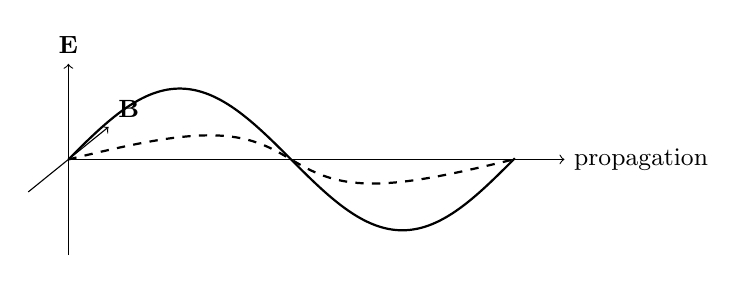
\begin{tikzpicture}[
  scale=0.9,
  x={(1cm,0cm)},
  y={(0cm,1cm)},
  z={(0.42cm,0.34cm)}
]
\draw[->] (0,0,0) -- (7,0,0) node[right] {\small propagation};
\draw[->] (0,-1.35,0) -- (0,1.35,0) node[above] {\small \(\mathbf E\)};
\draw[->] (0,0,-1.35) -- (0,0,1.35) node[above right] {\small \(\mathbf B\)};
\draw[thick,smooth,variable=\x,domain=0:6.3,samples=100]
  plot ({\x},{sin(\x r)},0);
\draw[thick,dashed,smooth,variable=\x,domain=0:6.3,samples=100]
  plot ({\x},0,{sin(\x r)});
\end{tikzpicture}
\caption{在電磁波中，電場與磁場彼此垂直，且兩者都垂直於傳播方向。}
\end{figure}

普通可見光的振盪快得無法直接追蹤其交變場。若是波長極長的無線電波，振盪也會相應地慢得多。無論哪一種情況，同樣的橫波幾何關係都會產生干涉。

\section{波長、週期與頻率}

波長\(\lambda\)是空間距離：從振盪中的某一點出發，沿著波前進，直到經過一個完整週期後，同一相位再次出現。波長以公尺、公分或其他長度單位表示。

現在停在某個位置，觀察波經過。完成一個完整週期所需的時間稱為週期\(T\)。可見光的週期極短，大約是\(10^{-15}\,\mathrm{s}\)的量級；波長越長，週期也越長，波長越短，週期也越短。

波在一個週期內前進一個波長，因此速度為\(v\)的波滿足
\begin{equation}
v=\frac{\lambda}{T}.
\end{equation}
水波和聲波各有自己的傳播速度。對光而言，
\begin{equation}
c=\frac{\lambda}{T}.
\end{equation}
頻率\(f\)是單位時間內完成的週期數：
\begin{equation}
f=\frac{1}{T}.
\end{equation}
因此
\begin{equation}
\lambda f=c.
\end{equation}
知道波長或頻率其中之一，就能決定另一個。

\begin{figure}[h]
\centering
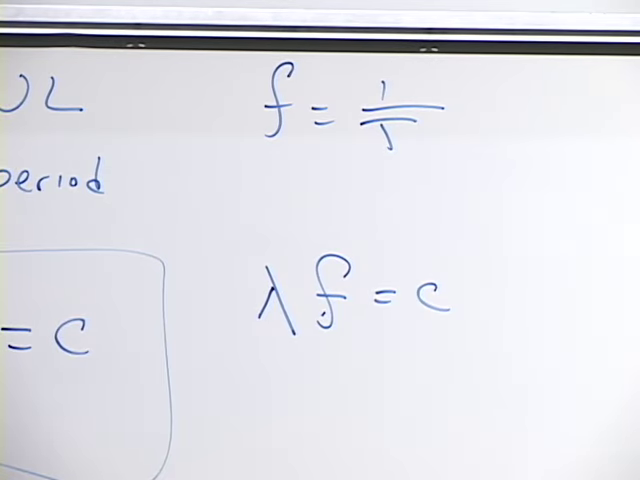
\includegraphics[width=0.68\textwidth]{lecture_01_figure_03.png}
\caption{對光波而言，\(f=1/T\)，而且\(\lambda f=c\)。}
\lectureframe{00:36:24}
\end{figure}

物理學家常以每秒弧度數，而非每秒完整週期數，來表示振盪速率。想像一個點沿圓周做等速運動。若該點每秒繞行\(f\)圈，而每圈包含\(2\pi\)弧度，其角頻率便是
\begin{equation}
\omega=2\pi f,
\qquad
\frac{\omega}{2\pi}=f.
\end{equation}
目前這只是定義；至於這種表示法實際上是否能減少\(2\pi\)因子的數目，稍後再談。

結合\(f=c/\lambda\)與\(\omega=2\pi f\)，得到
\begin{equation}
\omega=\frac{2\pi c}{\lambda},
\qquad
\omega\lambda=2\pi c.
\end{equation}
若考慮其他種類的波，式中的\(c\)就換成該波的傳播速度。

\begin{figure}[h]
\centering
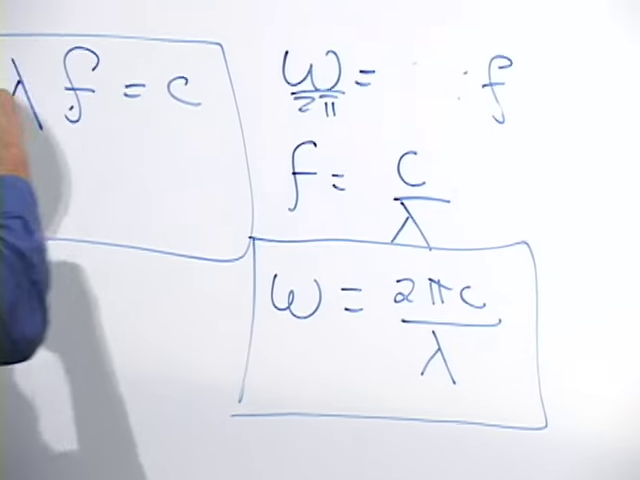
\includegraphics[width=0.68\textwidth]{lecture_01_figure_04.png}
\caption{對於\(\omega=2\pi f\)，光波滿足\(\omega=2\pi c/\lambda\)。}
\lectureframe{00:39:10}
\end{figure}

電磁輻射形成連續光譜。按波長由長至短排列，慣用名稱如下：
\begin{equation}
\begin{aligned}
\text{radio}
&\longrightarrow \text{microwave}
\longrightarrow \text{infrared}
\longrightarrow \text{visible}\\
&\longrightarrow \text{ultraviolet}
\longrightarrow \text{X ray}
\longrightarrow \text{gamma ray}.
\end{aligned}
\end{equation}
可見光只占其中一小段。各名稱所指區域之間的界線是約定俗成的，因此此處不必指定精確的分界波長。無線電波的波長可以極長；伽馬輻射則位於電磁光譜中波長極短的一端。現在問題變得鮮明：伽馬輻射在經典理論中是連續的場波，卻以離散的閃光事件被探測到。

\section{離散到達事件與波的機率}

從輻射的熱力學性質出發，普朗克和愛因斯坦得出結論：必須將光視為由離散單位構成。這個假想實驗能生動說明這一點，但不代表實際的歷史發現過程就是如此。

讓一束光照在螢幕上。一般強度下，光會形成一片看似連續的亮斑。在光束中放入部分不透明的衰減片，亮斑就會變暗。逐步加強衰減，每單位時間到達的光便越來越少。最後，亮斑的樣貌會改變：探測器記錄到的不再是連續變暗的光斑，而是一個個孤立事件。\footnote{此示意圖重現了講課影片中00:42:32至00:45:42之間講解的衰減實驗。}

\begin{figure}[h]
\centering
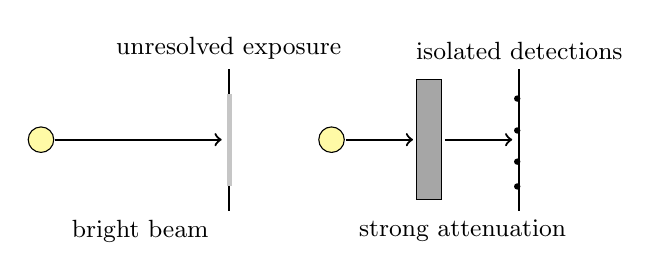
\begin{tikzpicture}[scale=0.9]
\begin{scope}
\draw[fill=yellow!35] (0,0) circle (0.18);
\draw[->,thick] (0.2,0) -- (2.55,0);
\draw[thick] (2.65,-1.0) -- (2.65,1.0);
\node[below] at (1.4,-1.0) {\small bright beam};
\end{scope}
\begin{scope}[xshift=4.1cm]
\draw[fill=yellow!35] (0,0) circle (0.18);
\draw[->,thick] (0.2,0) -- (1.15,0);
\draw[fill=gray!70] (1.2,-0.85) rectangle (1.55,0.85);
\draw[->,thick] (1.6,0) -- (2.55,0);
\draw[thick] (2.65,-1.0) -- (2.65,1.0);
\node[below] at (1.85,-1.0) {\small strong attenuation};
\end{scope}
\fill[gray!45] (2.62,-0.65) rectangle (2.70,0.65);
\foreach \y in {-0.66,-0.31,0.13,0.58}
  \fill (6.72,\y) circle (0.045);
\node[above] at (2.65,1.0) {\small unresolved exposure};
\node[above] at (6.75,1.0) {\small isolated detections};
\end{tikzpicture}
\caption{逐步衰減會降低探測率，直到看似連續的曝光分解為孤立的光子事件。}
\end{figure}

等待足夠久，這些事件累積起來後，會呈現出與原來光斑相同的空間分布。因此，明亮區域其實是許多個別到達事件疊加後、尚未分辨出的結果。這種低強度實驗確實可以進行，但它並不是最初促使人們提出光子假說的實驗。愛因斯坦提出光子概念，源於熱力學與光電效應方面的考量；衰減實驗則以特別直接的方式，呈現了光子概念的後果。

現在在光束中放入兩個孔徑，並降低光強，直到光子一次只來一個。每次探測都是一個局域事件。然而，探測多次之後，這些事件會逐漸形成干涉圖樣，包括明暗條紋。離散事件的到達具有隨機性，但其機率分布符合波動圖樣的預測。經典的波於是成為支配機率分布的波。

因此，波和粒子並非兩種分別屬於自然界不同部分的實體，而是同一個量子物體的兩種呈現方式。只把光描述成波，或只把光描述成粒子，都不夠充分。

電子帶來了相反方向的驚奇。人們早已接受電子是粒子，而且電子一次只會有一個抵達探測器；但若孔徑彼此夠近，電子也會逐漸形成干涉圖樣。阿爾法粒子的質量約為電子的八千倍，也遵循相同原理，只是實驗更加困難。甚至在巴克球中也觀察到干涉：這種分子由六十個碳原子組成，排列大致像一顆抽象化的足球。預期保齡球也適用相同原理，只是這種實驗在實際上極難進行。還可以進一步談到以病毒或活細胞進行的設想實驗，作為愈來愈大膽的例子。要理解波和粒子的描述如何相互契合，需要量子力學；眼前的任務則是找出粒子物理學所需的光子性質。

\section{光子能量}

光子是光的離散、不可分割單位。光會攜帶能量---陽光會加熱吸收它的物體---，所以每個光子都必須攜帶能量。單色波具有確定的波長和角頻率，其中每個光子的能量為
\begin{equation}
E_\gamma=\hbar\omega.
\end{equation}
若把連續波想像成由一小群機械質點組成，便容易產生誤解。可以確定的是這項實驗事實：局域探測事件遵循由波決定的分布，而能量則以不可分割的單位到達。

由於
\begin{equation}
\omega=\frac{2\pi c}{\lambda},
\end{equation}
波長越短，角頻率就越大，因此每個光子的能量也越高：
\begin{equation}
\lambda\downarrow
\quad\Longrightarrow\quad
\omega\uparrow
\quad\Longrightarrow\quad
E_\gamma\uparrow.
\end{equation}
單一無線電光子的能量很小。不過，無線電波束可以包含大量光子，因此仍能攜帶巨大的總能量。對於含有\(n\)個光子的單色脈衝，
\begin{equation}
E_{\text{pulse}}=n\hbar\omega,
\qquad
n=0,1,2,\ldots.
\end{equation}
總能量可能很大，但仍是單一光子能量的整數倍。

這個關係引出了將主導後續討論的實際問題：為什麼要建造愈來愈大的機器，才能觀察愈來愈小的東西？為什麼不能用小機器研究小物體？答案的前半已經出現：要解析更小的結構，就需要更短的波長；而短波長的量子具有更高的能量。

\section{靜止能量與不變質量}

粒子物理結合了量子力學與相對論。光子的關係式\(E_\gamma=\hbar\omega\)代表量子力學的一面；相對應的相對論基本事實則是
\begin{equation}
E_{\mathrm{rest}}=mc^2.
\end{equation}
這裡的限定很重要。較早的論述會區分\emph{靜質量}與依速度而變的\emph{動質量}。現代術語則以\emph{質量}表示物體的不變質量。運動會改變物體的能量，不會改變它的質量。無論處於何種運動狀態，每個電子的質量都相同；電子加速時，增加的是能量。因此，\(E=mc^2\)在這個形式下，表示一個有質量物體在其整體靜止的參考系中的能量。

物體不必連內部也完全靜止。一箱氣體放在秤上可以靜止不動，箱中分子卻仍朝各個方向快速運動。這些內部運動的能量屬於整箱氣體的靜止能量。先取一箱冷氣體，量出它的質量，再於箱子本身保持靜止時加入熱能。其靜止質量的變化為
\begin{equation}
\Delta m=\frac{\Delta E_{\mathrm{internal}}}{c^2}.
\end{equation}
質量增加時，重量和慣性也會增加。對普通的箱子而言，即使大幅升高溫度，這個效應仍小到無法用一般的秤察覺；效應微小並不改變這項原理。

更明確的例子是電子和正電子。兩者質量完全相同，電荷則相反。若它們起初都靜止並發生湮滅，能量會由光子帶走：
\begin{equation}
e^-+e^+\longrightarrow \text{photons}.
\end{equation}
初始能量為
\begin{equation}
E_{\mathrm{initial}}=2m_e c^2,
\end{equation}
這些能量不可能消失。單一粒子對產生的能量極少，因此要加熱一杯咖啡就需要極大量的粒子對；但個別湮滅事件直接呈現了這種轉換。

因此，對靜止物體而言，質量與能量是同一物理量，只是以不同單位表示。因子\(c^2\)是慣用質量單位與能量單位之間的換算因子，就像將公尺換算成公分時所用的數值因子。

\begin{classroomqa}
\lecturetimestamp{01:04:39}
\audiencequestion{將質量轉換為釋出的能量，需要某種機制嗎？}
\lecturerresponse{是的，這需要物理機制，但守恆定律已經限制了結果。即使尚未描述微觀的湮滅機制，起初電子--與正電子所具有的能量也必須在某處重新出現。因此，即使不詳細描述這種交互作用，能量守恆仍能決定答案中的重要部分。}
\end{classroomqa}

\section{量綱與單位的選擇}

在 SI 單位制中，光速的數值非常大，而普朗克常數的數值非常小。光子關係式已暗示了後者為何如此小：可見光的角頻率極高，單一光子的能量卻極低，因此在這套單位中，\(E_\gamma=\hbar\omega\)要求\(\hbar\)具有很小的數值。就數量級而言，
\begin{equation}
c\sim 10^8\ \mathrm{m\,s^{-1}},
\qquad
\hbar\sim 10^{-34}\ \mathrm{J\,s}.
\end{equation}
\editorialnote{此處只保留講課中提到的數量級，因為板書最後幾位數字不清楚。}
單位不可或缺：這兩個常數都不是沒有單位的單純小數。能量的量綱為
\begin{equation}
[E]=M L^2 T^{-2},
\end{equation}
又因為\(E_\gamma=\hbar\omega\)，且\([\omega]=T^{-1}\)，所以普朗克常數的量綱為
\begin{equation}
[\hbar]=[E]T=M L^2 T^{-1}.
\end{equation}

稱\(c\)的數值大、\(\hbar\)的數值小，已經預設了所採用的單位。速度以英尺每小時表示時，\(c\)的數值會不同於以公尺每秒表示時的數值。若以光年每年或光秒每秒為單位，光速的數值就是一。同樣地，適當配合質量、長度和時間單位，也可以令\(\hbar=1\)。

我們熟悉的單位制是沿用下來的慣例，並非自然界特別指定的單位。一英里等於5280英尺，一英石等於十四磅；馬匹以掌為單位量測高度，功率則可以馬力表示。公制單位較有系統，但其尺度仍是人為選擇。基礎物理中，沒有任何因素特別指定公尺、秒或公斤。

長度、時間和質量提供三種彼此獨立的基本單位選擇：
\begin{equation}
L,\qquad T,\qquad M.
\end{equation}
其他力學單位都可以由這些單位組合而成。適合的選擇取決於問題。在天文物理中，太陽質量很方便；在核物理中，質子質量可能更方便；在相對論天文學中，使用光年和年能讓公式更簡潔。有了三種獨立的選擇，就能為三個彼此獨立、具有量綱的常數指定方便的數值。天文物理、原子物理和粒子物理不必採用相同的選擇。

在粒子物理中，有兩種特別實用的慣例：
\begin{equation}
c=1,
\qquad
\hbar=1.
\end{equation}
剩下的單位沒有同樣突出的粒子質量可供選用。可以任意將質子質量、希格斯玻色子質量或{\proseunicodefont μ}子質量定為一，但那不過是讓眾多粒子中的某一種享有特殊地位。

那麼，為什麼選\(c\)和\(\hbar\)？乍看之下，或許是因為它們出現在許多方程中。但出現頻繁還不足以構成理由：質子質量也出現在許多方程中，質子的大小亦然。\(c\)和\(\hbar\)的特別之處，在於它們具有普適性。

常數\(c\)和\(\hbar\)的性質不同。速度\(c\)限制著所有物理物體：有質量的物體可以接近這個速度，卻不能被加速到超越它。普朗克常數則透過數量級的不確定性關係，限制所有量子物體：
\begin{equation}
\Delta x\,\Delta p\gtrsim\hbar.
\end{equation}
這兩項陳述都沒有特別指向某一種粒子。正因為具有普適性，\(c=1\)和\(\hbar=1\)才是自然的選擇。

質子無法提供同樣普適的尺度。它只是眾多物體中的一種。將質子質量定為一，並不比將銣原子的質量定為一更具基本性；電子、希格斯玻色子和{\proseunicodefont μ}子也有同樣的問題。

電荷看似能提供另一個普適量，但在\(c\)和\(\hbar\)歸一化之後，具有物理意義的電磁耦合是無量綱的。改變單位可以讓電磁公式中的有量綱常數轉移位置，卻無法改變真正無量綱的耦合。

重力提供了一個有量綱的普適常數。以牛頓力學的形式表示，兩個質量之間的力，其大小為
\begin{equation}
F=G\frac{m_1m_2}{r^2}.
\end{equation}
所有質量都參與重力作用，但電中性物體不一定會受到電力作用。因此，\(G\)具有所需的普適性。不過，對一般粒子物理而言，以它作為單位標準並不實用，因為在此處討論的計算中，已知基本粒子之間的引力可以忽略不計。

\begin{classroomqa}
\lecturetimestamp{01:20:34}
\audiencequestion{直接忽略 \(G\)合理嗎？在極高能量下，基本粒子可能不會如同這裡假設的那樣遵循經典重力。}
\lecturerresponse{單一粒子確實會受到地球重力場的作用：粒子會在這個場中下落。粒子彼此之間的重力作用尚未直接測量，因此在這個層次上，普適性假設仍可受到質疑。這裡省略 \(G\)，直接原因是實務考量，而非認定它絕對不存在：在一般粒子物理實驗與方程式中，重力的貢獻微不足道。}
\end{classroomqa}

\begin{classroomqa}
\lecturetimestamp{01:22:01}
\audiencequestion{能否以電磁作用取代重力，作為第三種設定單位的約定？}
\lecturerresponse{可以。可以選用一種電磁單位制，將電荷或庫侖定律中的常數正規化。確實有人採用這類約定。電子彼此排斥而非吸引，但這個符號差異不妨礙這種選擇；只是這裡不採用這種約定。}
\end{classroomqa}

\begin{classroomqa}
\lecturetimestamp{01:23:06}
\audiencequestion{將 \(c\) 和 \(\hbar\) 設為一之後，電荷就是無因次的嗎？}
\lecturerresponse{是的。與電荷平方相關的無因次量約為 \(1/137\)。確切的約定及這個數的意義可以留待稍後討論；這裡要強調的是，它是無因次的。}
\end{classroomqa}

\begin{classroomqa}
\lecturetimestamp{01:23:37}
\audiencequestion{可以選擇將庫侖常數作為第三個設為一的常數嗎？}
\lecturerresponse{可以將它吸收到電磁單位制的約定中。但這種選擇無法將無因次耦合常數 \(1/137\) 變成一，因為改變單位不會改變無因次的數值。這裡並未主張採用這種約定有什麼特別好處。}
\end{classroomqa}

\section{自然單位制中的方程式與參考系}

在 \(c=1\) 的單位制中，有質量物體的靜止能量關係式變為
\begin{equation}
E_{\mathrm{rest}}=m.
\end{equation}
在 \(\hbar=1\) 的單位制中，光子的關係式變為
\begin{equation}
E_\gamma=\omega.
\end{equation}
需要以慣用單位表示數值大小時，隨時可以恢復這些常數。

\begin{figure}[h]
\centering
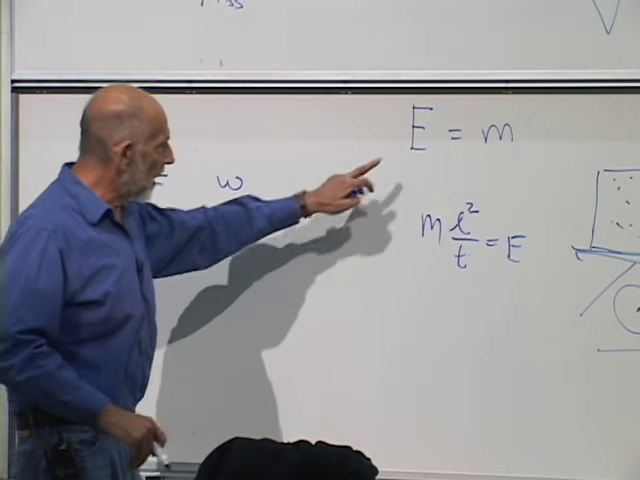
\includegraphics[width=0.72\textwidth]{lecture_01_figure_05.png}
\caption{在 \(c=1\) 的單位制中，靜止的有質量物體，其靜止能量為 \(E=m\)。}
\lectureframe{01:25:40}
\end{figure}

這些公式看起來相似，意義卻不同。在 \(E_{\mathrm{rest}}=m\) 中，\(E\) 是有質量物體的靜止能量。光子沒有質量，也無法靜止，因此它的能量不是靜止能量。關係式 \(E_\gamma=\omega\) 描述的是運動中的無質量量子所具有的能量。

\begin{classroomqa}
\lecturetimestamp{01:26:07}
\audiencequestion{既然靜止總是相對於某個參考物而言，而且實驗室本身也不是絕對靜止的，\emph{靜止}究竟是什麼意思？}
\lecturerresponse{靜止是相對於所選參考系來定義的。如果杯子相對於實驗室靜止，那麼在實驗室參考系中，當 \(c=1\) 時，它的能量就是它的質量，不含整體運動所造成的動能。另一位從杯子旁經過的觀察者，則會認為杯子也具有動能。不同觀察者通常會為同一物體或光子測得不同的能量；能量取決於參考系，這並不需要假設存在絕對靜止。}
\end{classroomqa}

現在可以重新檢視角頻率的約定。寫成 \(E_\gamma=\hbar\omega\) 很簡潔，但先前引入 \(\omega=2\pi f\) 時，還多出了一個 \(2\pi\) 因子。

\begin{classroomqa}
\lecturetimestamp{01:28:13}
\audiencequestion{為什麼要使用以弧度每秒為單位的角頻率 \(\omega\)，而不用看似更簡單的每秒完整週期數？}
\lecturerresponse{這個選擇部分出於歷史因素；至於數學上的理由，答案並非顯而易見，而是取決於實際使用。這裡提供的答案仍屬暫定：分別用 \(f\) 和 \(\omega\) 寫出相關方程式，再看看哪種約定留下的 \(2\pi\) 因子較少。不論如何選擇，\(2\pi\) 因子都不可能在所有地方消失。有人也提出，這可能與複指數記號有關，但這裡不再深入討論。}
\end{classroomqa}

\begin{classroomqa}
\lecturetimestamp{01:29:51}
\audiencequestion{能否將兩個粒子加速，直到它們之間的重力作用變得重要？}
\lecturerresponse{原則上可以。實際上，目前的加速器離這個範圍還非常遙遠。答案也取決於「粒子」的定義：宏觀的受重力物體並非這裡所討論的基本粒子。}
\end{classroomqa}

\begin{classroomqa}
\lecturetimestamp{01:30:27}
\audiencequestion{什麼可以作為正電子的來源？}
\lecturerresponse{高能碰撞可以產生正電子。有些核過程與衰變也會產生正電子。}
\end{classroomqa}

\begin{classroomqa}
\lecturetimestamp{01:30:53}
\audiencequestion{這裡使用的自然單位是普朗克時間和普朗克距離嗎？}
\lecturerresponse{不是。當 \(G\)、\(c\) 和 \(\hbar\) 都設為一時，便得到普朗克單位。由此定義的普朗克長度遠小於一般粒子物理涉及的長度尺度，因此不適合作為這裡的量尺。當重力、量子力學和相對論都同時重要時，例如在黑洞物理、宇宙學或量子重力中，這類單位才自然合用。若重力可以忽略，只將 \(c\) 和 \(\hbar\) 設為一會更實用。}
\end{classroomqa}

\section{動量、光與解析度}

接下來要介紹的基本概念是動量。物體靜止時沒有動量，儘管它具有非零的靜止能量 \(mc^2\)。物體一旦運動，通常就會帶有動量。動量和能量一樣，在碰撞中守恆：兩個物體碰撞前後，總向量動量相同。凡是受守恆定律約束的物理量，都值得特別留意。

動量是向量，方向沿著運動方向。對非相對論性物體，
\begin{equation}
\mathbf p=m\mathbf v.
\end{equation}
這不是一般的相對論公式，不能直接用於光。

不過，光也攜帶動量和能量。一般光所產生的推力極小，動量很難察覺；但強烈的雷射脈衝可以傳遞相當大的衝量。例如，利佛摩爾的大型雷射可以利用輻射攜帶的動量，將物質向內推。

考慮一個準直程度足夠高、光線幾乎沿著單一軸向傳播的脈衝。真實光束可能有一定的角度散布，各部分沿著略有差異的方向傳播；但對理想的準直光束而言，動量方向沿著光束，大小為
\begin{equation}
p=\frac{E}{c},
\qquad\text{or equivalently}\qquad
E=cp.
\end{equation}
這裡將此關係視為相對論中的一項事實，而不加以證明。以下的量綱檢查只能確認它的單位與一般動量的單位相符：
\begin{equation}
\left[\frac{E}{c}\right]
=
\frac{M L^2 T^{-2}}{L T^{-1}}
=
M L T^{-1}
=
[m v]
=
[p].
\end{equation}
這項量綱比較並未賦予光靜止質量。光子的質量為零；它之所以具有動量，是因為它攜帶能量，並以 \(c\) 運動。

\(\mathbf p\) 的方向就是傳播方向。它的大小通常難以測量，因為 \(c\) 出現在分母。光束可以輕易透過加熱或蒸發物質，展現所攜帶的能量；相較之下，它造成的機械推力小得多。不過，只要強度夠大，這股推力也可以變得很大。

對單一光子而言，
\begin{align}
p_\gamma
&=\frac{E_\gamma}{c}\\
&=\frac{\hbar\omega}{c}.
\end{align}
要改用波長表示，必須仔細回到波的關係式。由於
\begin{equation}
f\lambda=c,
\qquad
\omega=2\pi f,
\end{equation}
正確的關係式是
\begin{equation}
\omega\lambda=2\pi c,
\qquad
\omega=\frac{2\pi c}{\lambda}.
\end{equation}
若沒有先寫出定義，\(2\pi\) 這個因子很容易顛倒。重新從 \(f\lambda=c\) 和 \(f=\omega/(2\pi)\) 出發，就能釐清：
\begin{equation}
\frac{\omega}{2\pi}\lambda=c
\quad\Longrightarrow\quad
\omega\lambda=2\pi c.
\end{equation}
代入後得到
\begin{align}
p_\gamma
&=\frac{\hbar}{c}\frac{2\pi c}{\lambda}\\
&=\frac{2\pi\hbar}{\lambda}\\
&=\frac{h}{\lambda}.
\end{align}

\begin{classroomqa}
\lecturetimestamp{01:42:38}
\audiencequestion{\(2\pi\hbar\)等於 \(h\) 嗎？}
\lecturerresponse{是的。依定義，\(h=2\pi\hbar\)，所以 \(p_\gamma=2\pi\hbar/\lambda\) 與 \(p_\gamma=h/\lambda\) 相同。無論選用哪種頻率約定，某處都會重新出現 \(2\pi\) 因子。}
\end{classroomqa}

波長越短，光子的動量越大。無線電波光子的波長很長，動量極小；伽馬射線光子的波長很短，造成的衝擊大得多。單一光子帶來的宏觀衝量仍然很小，但其動量遠大於無線電波光子。它的能量也比較大，因為 \(E_\gamma=cp_\gamma\)。

這個關係說明了為什麼要觀察越小的物體，就需要越大型的機器。若用遠長於人頭的波長拍照，影像只會模糊一片。要分辨五官，波長必須短於頭部尺寸；要看清一根頭髮，波長必須與髮絲的粗細相當或更短；要解析原子的結構，探測波長不能大於原子：
\begin{equation}
\lambda_{\mathrm{probe}}\lesssim
\text{size of the structure to be resolved}.
\end{equation}
因此，結構越小，所需的波長越短；波長越短，所需的動量和能量就越大。探測粒子不一定是光子；其他種類的高能粒子也遵循相同的波長與動量之間的量子關係。要產生這些粒子，必須用加速器將越來越多的能量傳給每個粒子。\(p_\gamma=h/\lambda\) 和 \(E_\gamma=\hbar\omega\) 這兩個關係式串起了整個論證：提高探測能量會增加動量並縮短波長。

近一個世紀以來，粒子物理學反覆呈現相同的脈絡：能量越高、動量越大、波長越短，空間解析度也越精細。

\begin{classroomqa}
\lecturetimestamp{01:46:57}
\audiencequestion{波長在理論上有沒有下限？}
\lecturerresponse{可能有。在普朗克長度附近，預期會出現新的現象，但這個答案仍屬暫定。即使空間解析度真的在那個尺度觸及下限，它仍比大型強子對撞機目前探測的距離小約十七個數量級；因此，現今實驗距離那個尺度還非常遙遠。}
\end{classroomqa}

沿著同一套推理，可以粗略看出加速器的尺度與它能解析的尺度之間的關係。

\begin{classroomqa}
\lecturetimestamp{01:48:02}
\audiencequestion{波長，或者說所解析的尺寸，是否大致與加速器的尺寸成反比？}
\lecturerresponse{大致如此，前提是加速粒子所用的最大電場，以及引導粒子所用的磁場，都受限於現有設備。加速梯度表示每單位長度所增加的能量。對於長度為 \(L\)、加速梯度 \(\mathcal G\) 大致固定的直線加速器，
\[
E_{\mathrm{beam}}\sim \mathcal G L.
\]
在超相對論能量下，可解析的波長與能量成反比，因此加長直線加速器，大致會以相應的反比因子提升解析度。這只是啟發式的尺度關係，並非精確定律。環形加速器可以讓粒子反覆通過同一設備，但帶電粒子在彎轉時會輻射並損失能量。}
\end{classroomqa}

\begin{classroomqa}
\lecturetimestamp{01:49:47}
\audiencequestion{要達到普朗克長度，加速器得有多大？}
\lecturerresponse{按照這個粗略的尺度關係，加速器必須比 CERN 的加速器長約十七個數量級。這還不到宇宙的尺度，但大致相當於星系的尺度。}
\end{classroomqa}

\begin{classroomqa}
\lecturetimestamp{01:50:09}
\audiencequestion{最高能量宇宙射線的能量，與對撞機能量相比如何？}
\lecturerresponse{單一宇宙射線的能量可以遠高於實驗室能量。為了作數值比較，取一個實驗室能量約為 \(10^{21}\,\mathrm{eV}=10^{12}\,\mathrm{GeV}\) 的極高能宇宙射線。然而，宇宙射線撞擊的是在實驗室中靜止的靶；對撞機則讓兩束高能粒子束迎頭碰撞。更重要的是，進行有用的實驗需要足夠的通量，也就是大量粒子和許多受控良好的碰撞。單一宇宙射線可能打不中相關的靶，或只產生一個難以推知任何結果的事件。一項刻意誇大的石油當量估算指出，要讓一座有用的星系尺度加速器運轉，每秒所需的石油供應量約為一百兆桶。這個估算是要說明，取得足夠的碰撞統計量，至少會和加速器的長度一樣，構成嚴重障礙。}
\end{classroomqa}

\editorialnote{來源中的石油當量估算前後不一致：先提出一個數值，接著又說約為每秒 \(10^{14}\) 桶；後來再次敘述時，則給出每秒 \(10^{11}\) 桶。這裡保留兩種數量級，沒有逕自將它們調整成一致。}

這些都是實際的距離尺度，不只是形式上的尺度。實際難題在於，如何不建造星系尺度的加速器，也不提供其荒誕的所需功率，就能探測這些尺度。

\begin{classroomqa}
\lecturetimestamp{01:52:55}
\audiencequestion{應如何將 LHC 的能量與能量為 \(10^{12}\,\mathrm{GeV}\) 的宇宙射線相比？}
\lecturerresponse{對於實驗室能量為 \(E_{\mathrm{lab}}\)、撞擊質量為 \(m_{\mathrm{target}}\) 的靜止靶的超相對論性入射粒子，質心能量的尺度關係為
\[
E_{\mathrm{cm}}\simeq
\sqrt{2m_{\mathrm{target}}c^2E_{\mathrm{lab}}}.
\]
\editorialnote{這裡列出的固定靶公式，明確呈現了問答中所述的平方根尺度關係。}
因此，在靶的質量固定時，有效碰撞能量只會隨入射粒子能量的平方根增加。所以，能量為 \(10^{12}\,\mathrm{GeV}\) 的宇宙射線，約相當於兩束迎頭相撞、每束能量約為 \(10^6\,\mathrm{GeV}\) 的粒子束，而不是每束 \(10^{12}\,\mathrm{GeV}\)。宇宙射線的能量仍可能超過地面對撞機，但其通量極低，無法用於系統性的受控實驗。}
\end{classroomqa}